% R42: Pareto Frontier — Accuracy vs Retrieval Efficiency
% Usage: % R42: Pareto Frontier — Accuracy vs Retrieval Efficiency
% Usage: % R42: Pareto Frontier — Accuracy vs Retrieval Efficiency
% Usage: % R42: Pareto Frontier — Accuracy vs Retrieval Efficiency
% Usage: \input{figures/pareto_frontier.tex} inside a figure environment
% Requires: \usepackage{pgfplots} and \pgfplotsset{compat=1.18}

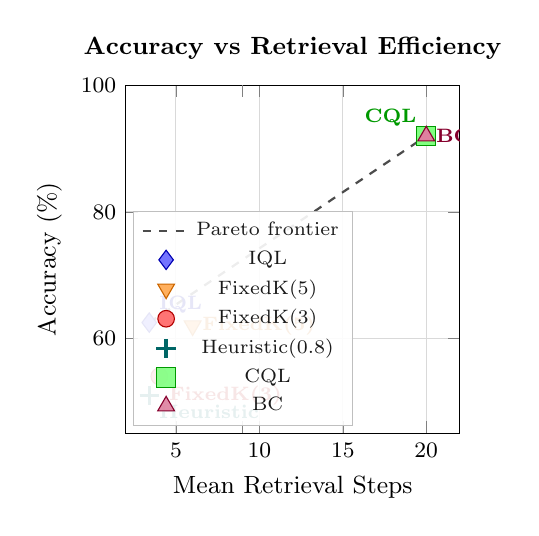
\begin{tikzpicture}
\begin{axis}[
    width=0.48\textwidth,
    height=6cm,
    xlabel={Mean Retrieval Steps},
    ylabel={Accuracy (\%)},
    title={\textbf{Accuracy vs Retrieval Efficiency}},
    title style={font=\small},
    label style={font=\small},
    tick label style={font=\footnotesize},
    xmin=2, xmax=22,
    ymin=45, ymax=100,
    grid=major,
    grid style={gray!30},
    legend style={
        at={(0.02,0.02)},
        anchor=south west,
        font=\scriptsize,
        draw=gray!50,
        fill=white,
        fill opacity=0.9,
    },
    % Broken axis effect via extra x ticks
    extra x ticks={9},
    extra x tick labels={},
    extra x tick style={grid=none},
]

% Pareto frontier line (IQL -> CQL)
\addplot[
    dashed, thick, color=black!70, mark=none,
] coordinates {
    (3.4, 62.5)
    (20.0, 92.0)
};
\addlegendentry{Pareto frontier}

% IQL
\addplot[only marks, mark=diamond*, mark size=3.5pt,
    color=blue!70!black, fill=blue!60] coordinates {(3.4, 62.5)};
\addlegendentry{IQL}
\node[above right, font=\scriptsize\bfseries, color=blue!70!black]
    at (axis cs:3.4,62.5) {IQL};

% FixedK(5)
\addplot[only marks, mark=triangle*, mark size=3.5pt, mark options={rotate=180},
    color=orange!80!black, fill=orange!70] coordinates {(6.0, 62.0)};
\addlegendentry{FixedK(5)}
\node[right, font=\scriptsize\bfseries, color=orange!80!black]
    at (axis cs:6.0,62.0) {FixedK(5)};

% FixedK(3)
\addplot[only marks, mark=*, mark size=3pt,
    color=red!70!black, fill=red!60] coordinates {(4.0, 54.0)};
\addlegendentry{FixedK(3)}
\node[below right, font=\scriptsize\bfseries, color=red!70!black]
    at (axis cs:4.0,54.0) {FixedK(3)};

% Heuristic(0.8)
\addplot[only marks, mark=+, mark size=3.5pt, very thick,
    color=teal!80!black] coordinates {(3.4, 51.0)};
\addlegendentry{Heuristic(0.8)}
\node[below right, font=\scriptsize\bfseries, color=teal!80!black]
    at (axis cs:3.4,51.0) {Heuristic};

% CQL
\addplot[only marks, mark=square*, mark size=3.5pt,
    color=green!60!black, fill=green!50] coordinates {(20.0, 92.0)};
\addlegendentry{CQL}
\node[above left, font=\scriptsize\bfseries, color=green!60!black]
    at (axis cs:20.0,92.0) {CQL};

% BC
\addplot[only marks, mark=triangle*, mark size=3.5pt,
    color=purple!70!black, fill=purple!50] coordinates {(20.0, 92.0)};
\addlegendentry{BC}
\node[right, font=\scriptsize\bfseries, color=purple!70!black]
    at (axis cs:20.0,92.0) {BC};

\end{axis}
\end{tikzpicture}
 inside a figure environment
% Requires: \usepackage{pgfplots} and \pgfplotsset{compat=1.18}

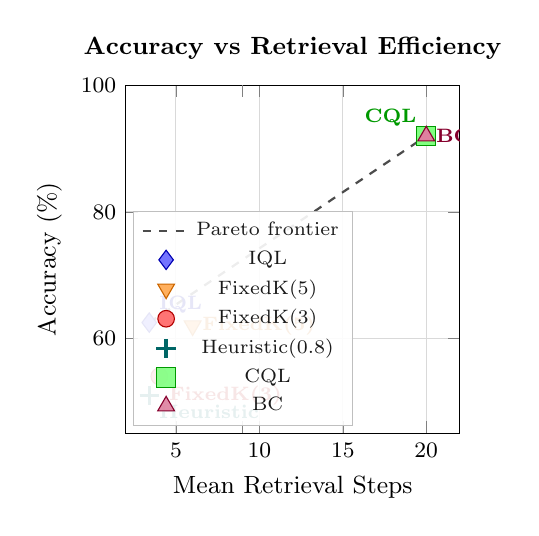
\begin{tikzpicture}
\begin{axis}[
    width=0.48\textwidth,
    height=6cm,
    xlabel={Mean Retrieval Steps},
    ylabel={Accuracy (\%)},
    title={\textbf{Accuracy vs Retrieval Efficiency}},
    title style={font=\small},
    label style={font=\small},
    tick label style={font=\footnotesize},
    xmin=2, xmax=22,
    ymin=45, ymax=100,
    grid=major,
    grid style={gray!30},
    legend style={
        at={(0.02,0.02)},
        anchor=south west,
        font=\scriptsize,
        draw=gray!50,
        fill=white,
        fill opacity=0.9,
    },
    % Broken axis effect via extra x ticks
    extra x ticks={9},
    extra x tick labels={},
    extra x tick style={grid=none},
]

% Pareto frontier line (IQL -> CQL)
\addplot[
    dashed, thick, color=black!70, mark=none,
] coordinates {
    (3.4, 62.5)
    (20.0, 92.0)
};
\addlegendentry{Pareto frontier}

% IQL
\addplot[only marks, mark=diamond*, mark size=3.5pt,
    color=blue!70!black, fill=blue!60] coordinates {(3.4, 62.5)};
\addlegendentry{IQL}
\node[above right, font=\scriptsize\bfseries, color=blue!70!black]
    at (axis cs:3.4,62.5) {IQL};

% FixedK(5)
\addplot[only marks, mark=triangle*, mark size=3.5pt, mark options={rotate=180},
    color=orange!80!black, fill=orange!70] coordinates {(6.0, 62.0)};
\addlegendentry{FixedK(5)}
\node[right, font=\scriptsize\bfseries, color=orange!80!black]
    at (axis cs:6.0,62.0) {FixedK(5)};

% FixedK(3)
\addplot[only marks, mark=*, mark size=3pt,
    color=red!70!black, fill=red!60] coordinates {(4.0, 54.0)};
\addlegendentry{FixedK(3)}
\node[below right, font=\scriptsize\bfseries, color=red!70!black]
    at (axis cs:4.0,54.0) {FixedK(3)};

% Heuristic(0.8)
\addplot[only marks, mark=+, mark size=3.5pt, very thick,
    color=teal!80!black] coordinates {(3.4, 51.0)};
\addlegendentry{Heuristic(0.8)}
\node[below right, font=\scriptsize\bfseries, color=teal!80!black]
    at (axis cs:3.4,51.0) {Heuristic};

% CQL
\addplot[only marks, mark=square*, mark size=3.5pt,
    color=green!60!black, fill=green!50] coordinates {(20.0, 92.0)};
\addlegendentry{CQL}
\node[above left, font=\scriptsize\bfseries, color=green!60!black]
    at (axis cs:20.0,92.0) {CQL};

% BC
\addplot[only marks, mark=triangle*, mark size=3.5pt,
    color=purple!70!black, fill=purple!50] coordinates {(20.0, 92.0)};
\addlegendentry{BC}
\node[right, font=\scriptsize\bfseries, color=purple!70!black]
    at (axis cs:20.0,92.0) {BC};

\end{axis}
\end{tikzpicture}
 inside a figure environment
% Requires: \usepackage{pgfplots} and \pgfplotsset{compat=1.18}

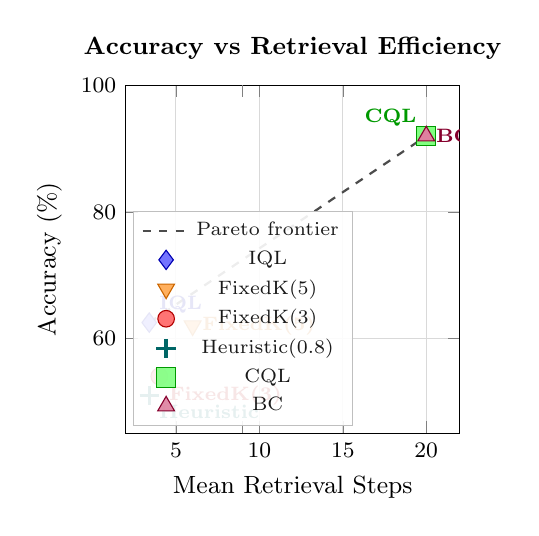
\begin{tikzpicture}
\begin{axis}[
    width=0.48\textwidth,
    height=6cm,
    xlabel={Mean Retrieval Steps},
    ylabel={Accuracy (\%)},
    title={\textbf{Accuracy vs Retrieval Efficiency}},
    title style={font=\small},
    label style={font=\small},
    tick label style={font=\footnotesize},
    xmin=2, xmax=22,
    ymin=45, ymax=100,
    grid=major,
    grid style={gray!30},
    legend style={
        at={(0.02,0.02)},
        anchor=south west,
        font=\scriptsize,
        draw=gray!50,
        fill=white,
        fill opacity=0.9,
    },
    % Broken axis effect via extra x ticks
    extra x ticks={9},
    extra x tick labels={},
    extra x tick style={grid=none},
]

% Pareto frontier line (IQL -> CQL)
\addplot[
    dashed, thick, color=black!70, mark=none,
] coordinates {
    (3.4, 62.5)
    (20.0, 92.0)
};
\addlegendentry{Pareto frontier}

% IQL
\addplot[only marks, mark=diamond*, mark size=3.5pt,
    color=blue!70!black, fill=blue!60] coordinates {(3.4, 62.5)};
\addlegendentry{IQL}
\node[above right, font=\scriptsize\bfseries, color=blue!70!black]
    at (axis cs:3.4,62.5) {IQL};

% FixedK(5)
\addplot[only marks, mark=triangle*, mark size=3.5pt, mark options={rotate=180},
    color=orange!80!black, fill=orange!70] coordinates {(6.0, 62.0)};
\addlegendentry{FixedK(5)}
\node[right, font=\scriptsize\bfseries, color=orange!80!black]
    at (axis cs:6.0,62.0) {FixedK(5)};

% FixedK(3)
\addplot[only marks, mark=*, mark size=3pt,
    color=red!70!black, fill=red!60] coordinates {(4.0, 54.0)};
\addlegendentry{FixedK(3)}
\node[below right, font=\scriptsize\bfseries, color=red!70!black]
    at (axis cs:4.0,54.0) {FixedK(3)};

% Heuristic(0.8)
\addplot[only marks, mark=+, mark size=3.5pt, very thick,
    color=teal!80!black] coordinates {(3.4, 51.0)};
\addlegendentry{Heuristic(0.8)}
\node[below right, font=\scriptsize\bfseries, color=teal!80!black]
    at (axis cs:3.4,51.0) {Heuristic};

% CQL
\addplot[only marks, mark=square*, mark size=3.5pt,
    color=green!60!black, fill=green!50] coordinates {(20.0, 92.0)};
\addlegendentry{CQL}
\node[above left, font=\scriptsize\bfseries, color=green!60!black]
    at (axis cs:20.0,92.0) {CQL};

% BC
\addplot[only marks, mark=triangle*, mark size=3.5pt,
    color=purple!70!black, fill=purple!50] coordinates {(20.0, 92.0)};
\addlegendentry{BC}
\node[right, font=\scriptsize\bfseries, color=purple!70!black]
    at (axis cs:20.0,92.0) {BC};

\end{axis}
\end{tikzpicture}
 inside a figure environment
% Requires: \usepackage{pgfplots} and \pgfplotsset{compat=1.18}

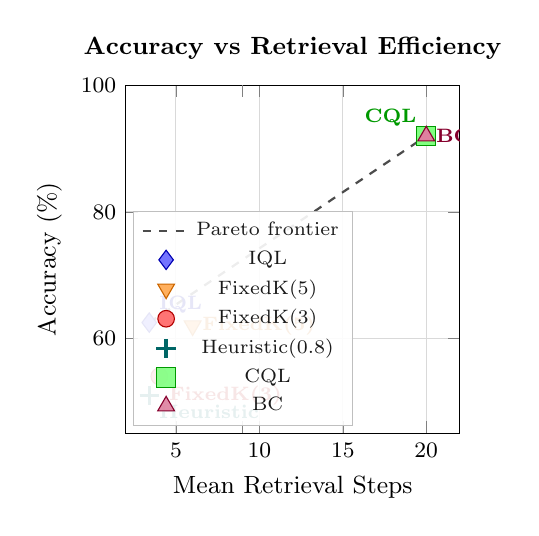
\begin{tikzpicture}
\begin{axis}[
    width=0.48\textwidth,
    height=6cm,
    xlabel={Mean Retrieval Steps},
    ylabel={Accuracy (\%)},
    title={\textbf{Accuracy vs Retrieval Efficiency}},
    title style={font=\small},
    label style={font=\small},
    tick label style={font=\footnotesize},
    xmin=2, xmax=22,
    ymin=45, ymax=100,
    grid=major,
    grid style={gray!30},
    legend style={
        at={(0.02,0.02)},
        anchor=south west,
        font=\scriptsize,
        draw=gray!50,
        fill=white,
        fill opacity=0.9,
    },
    % Broken axis effect via extra x ticks
    extra x ticks={9},
    extra x tick labels={},
    extra x tick style={grid=none},
]

% Pareto frontier line (IQL -> CQL)
\addplot[
    dashed, thick, color=black!70, mark=none,
] coordinates {
    (3.4, 62.5)
    (20.0, 92.0)
};
\addlegendentry{Pareto frontier}

% IQL
\addplot[only marks, mark=diamond*, mark size=3.5pt,
    color=blue!70!black, fill=blue!60] coordinates {(3.4, 62.5)};
\addlegendentry{IQL}
\node[above right, font=\scriptsize\bfseries, color=blue!70!black]
    at (axis cs:3.4,62.5) {IQL};

% FixedK(5)
\addplot[only marks, mark=triangle*, mark size=3.5pt, mark options={rotate=180},
    color=orange!80!black, fill=orange!70] coordinates {(6.0, 62.0)};
\addlegendentry{FixedK(5)}
\node[right, font=\scriptsize\bfseries, color=orange!80!black]
    at (axis cs:6.0,62.0) {FixedK(5)};

% FixedK(3)
\addplot[only marks, mark=*, mark size=3pt,
    color=red!70!black, fill=red!60] coordinates {(4.0, 54.0)};
\addlegendentry{FixedK(3)}
\node[below right, font=\scriptsize\bfseries, color=red!70!black]
    at (axis cs:4.0,54.0) {FixedK(3)};

% Heuristic(0.8)
\addplot[only marks, mark=+, mark size=3.5pt, very thick,
    color=teal!80!black] coordinates {(3.4, 51.0)};
\addlegendentry{Heuristic(0.8)}
\node[below right, font=\scriptsize\bfseries, color=teal!80!black]
    at (axis cs:3.4,51.0) {Heuristic};

% CQL
\addplot[only marks, mark=square*, mark size=3.5pt,
    color=green!60!black, fill=green!50] coordinates {(20.0, 92.0)};
\addlegendentry{CQL}
\node[above left, font=\scriptsize\bfseries, color=green!60!black]
    at (axis cs:20.0,92.0) {CQL};

% BC
\addplot[only marks, mark=triangle*, mark size=3.5pt,
    color=purple!70!black, fill=purple!50] coordinates {(20.0, 92.0)};
\addlegendentry{BC}
\node[right, font=\scriptsize\bfseries, color=purple!70!black]
    at (axis cs:20.0,92.0) {BC};

\end{axis}
\end{tikzpicture}
